\vspace{-5pt}
\section{Model} \label{sec:model}


%This paper is concerned with the decision mechanism of determining optimal load shedding subject to a generation capacity constraint on the total satisfiable power demand. 
%Throughout this paper, $\nu^{\rm R} \triangleq {\rm Re}(\nu)$ is sometimes denoted as the real part and $\nu^{\rm I} \triangleq {\rm Im}(\nu)$ as the imaginary part of a given complex number $\nu$. %Also, interchangeably denote a complex number by a 2D-vector as well as a point in the complex plane. $|\nu|$ denotes the magnitude of complex number $\nu$.

%In event driven demand response, there may arise occasions of load \textit{shedding} in response to requests by the grid operators, due to emergent situations (e.g., power transmission failures) or planned maintenance. 
%For AC electric systems, the power is determined by periodic time-varying voltage and current, which give rise to both {\em active} power (that delivers work at loads) and {\em reactive} power (that continuously bounces back and forth between sources and loads). The combination of active power and reactive power is known as {\em apparent} power. The physical capacity of power generation is often expressed by apparent power. 
%It is vital to ensure that the total power usage is within the apparent power constraint. As in the literature, apparent power is represented by a complex number, whereas the real part represents the active power, and the imaginary part represents the reactive power.

To model the decision mechanism of determining load curtailment, two major scenarios are considered in this paper.
The first scenario considers customers submitting bids (i.e., valuations) to prevent their power demand from being curtailed. The objective is to maximize the total valuation of satisfiable customers. The second scenario considers paying customers compensations (or penalties) for their power interruption, which may be stipulated as a part of the usage contract. The objective is to minimize the total compensation paid to unsatisfiable customers. 

The two problems involving a decision at a particular time are formulated as follows.
\begin{enumerate}
 
\item
{\em Valuation-maximizing power allocation problem}: %\vspace{-5pt}
\begin{eqnarray}
\textsc{(maxPA)} & &  \displaystyle \max_{x_k \in \{0, 1 \}} \sum_{k\in{\cal N}}u_k x_k \label{DAP}\\
\text{subject to}& &  \displaystyle \Big|\sum_{k\in {\cal N}}S_k x_k\Big| \le C. \label{maxPA}
\end{eqnarray}
where ${\cal N}$ is the set of customers, $u_k$ is the valuation of $k$-th customer, $S_k = P_k + {\bf i} Q_k \in\CC$ is the {\em complex-valued} apparent power demand for $k$-th customer, $C \in\RR_+$ is a real-valued capacity of total apparent generation power. $x_k$ is a binary decision variable if the $k$-th customer's power demand is retained.


\item
{\em Compensation-minimizing power allocation problem}: %\vspace{-5pt}
\begin{eqnarray}
\textsc{(minPA)} & &  \displaystyle \min_{x_k \in \{0, 1 \}} \sum_{k\in{\cal N}}c_k (1-x_k) \label{DAP}\\
\text{subject to}& &  \displaystyle \Big|\sum_{k\in {\cal N}}S_k x_k\Big| \le C. \label{C1}
\end{eqnarray}
where $c_k$ is the compensation paid $k$-th customer. $(1-x_k)$ is a binary decision variable if the $k$-th customer's power demand is curtailed.

\end{enumerate}

While the preceding optimization problems are not entirely new, there lack efficient algorithms to compute the decisions with provable guarantees for a large number of customers. The reason is that these problems encompass a classical NP-hard problem (known as knapsack problem \cite{KSbook}). Specifically, {\sc maxPA} is equivalent to the classical knapsack problem when setting zero reactive power, namely, $Q_k = 0$ for all $k \in {\cal N}$. There is no known efficient algorithms that can compute the exact optimal solutions for any NP-hard problem. Furthermore, the incorporation of active and reactive power creates a harder problem than the classical knapsack problem \cite{CKM14}. Nonetheless, this paper provides efficient algorithms that compute solutions that are close to the optimal solution with a precise theoretical guarantee on the optimality gap. The efficient algorithms give scalable running time with the number of customers, enabling fast decisions for a large number of customers. 




%\begin{figure}[!htb]
%	\begin{center}
%		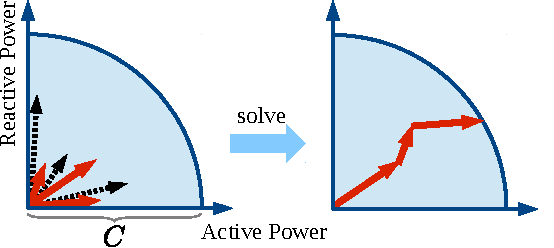
\includegraphics[scale=0.85]{fig/fig-sol-horizontal.pdf}
%	\end{center}
%\caption{The left figure shows the set of all demands $\{S_k(t)\}$. Red vectors represent a feasible solution to {\sc maxPA} such that the total magnitude of the red demands remain within radius $C$ as shown in the right figure.}
%	\label{fig:problem}
%\end{figure}  



%In particular, we will write {\sc maxPA}$[\phi_1,\phi_2]$ for the restriction of problem {\sc maxPA} subject to $\phi_1 \le \max_{k \in {\cal N}}{\rm arg}(S_k(t)) \le \phi_2$, where ${\rm arg}(S_k(t))\ge 0$ for all $k \in {\cal N}$ (see Fig.~\ref{fig:rotate} for an illustration). We remark that in realistic setting of power systems, the active power demand is positive (i.e., $P_k(t) \ge 0$), but the power factor (i.e., $\frac{d^{\rm R}_k}{|S_k(t)|}$) is bounded by a certain threshold \cite{NEC}, which is equivalent to restricting the argument of complex-valued demands. 
%\begin{figure}[!ht]
%	\begin{center}
%		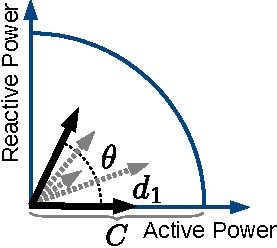
\includegraphics[scale=1]{fig/fig-angle.pdf}
%	\end{center}
%\caption{$\theta$ is the maximum angle between any pair of demands. }
%	\label{fig:rotate}
%\end{figure} 

%For complexity issues, we will need to specify how the input is described. Throughout the paper will assume that each of the demands is given by its real and imaginary components, represented as rational numbers\footnote{we may also consider other representations, such as the {\it polar representation}, and the conversion between the two representations can be done using standard numerical approximations}, and that the capacity parameter $C$ is also rational. 


The generation capacity $C(t)$ could be dynamically varying, and the decisions of load curtailment $(x_k(t))_{k \in {\cal N}}$ need to be determined from time to time. It is assumed that the decisions are triggered at every discrete timeslot $t$. 


\vspace{-5pt}
\subsection{Close-to-optimal Solutions}

Since the exact optimal solutions are computationally hard, this paper focuses on feasible solutions that are close to the optimal solutions. Furthermore, these close-to-optimal solutions are assured with a precise worst-case guarantee on the optimality gap. Some notations are defined as follows to characterize the optimality gap.
\\


\begin{definition}
For clarity, {\sc maxPA} is considered.
Let $ x^\ast_k $ be an optimal solution to {\sc maxPA} and $\OPT \triangleq \sum_{k\in{\cal N}}u_k x^\ast_k$ be the corresponding total valuation.
An approximation solution with $\alpha \in [0, 1]$ worst-case guarantee to {\sc maxPA} is a feasible solution $(\hat{x}_k)_{k \in {\cal N}} \in \{0, 1\}^n$ satisfying %\vspace{-5pt}
\begin{eqnarray}
& &   \displaystyle \sum_{k\in{\cal N}}u_k \hat{x}_k\ge \alpha \cdot \OPT \\
\text{and} & & \displaystyle \Big|\sum_{k\in{\cal N}}S_k \hat{x}_k\Big| \le C \label{C1'}.
\end{eqnarray}
\end{definition}


The worst-case guarantee is called {\em approximation ratio}, which characterizes the ratio between the optimal solution and the approximation solution. When $\alpha = 1$, this implies exact optimal solutions. In the subsequent sections, efficient algorithms are presented with definite worst-case guarantees.

First, a greedy approach is proposed that is capable of determining a close-to-optimal solution rapidly. The worst-case guarantee of this greedy approach depends on the maximum phase angle between any pair of power demand. The smaller phase angle produces a smaller optimality gap. 

Second, a one-dimensional projection algorithm is presented that projects the power demands represented by two-dimensional vector in complex plane to one-dimensional vectors, and utilizes a well-known approximation algorithm from knapsack problem to solve the problem. This approach requires more computations, and a longer running time. However, the worst-case guarantee is superior to that of the greedy approach. 

Finally, a hybrid approach is proposed that harnesses both approaches as a two-stage process, where the greedy approach is firstly utilized rapidly to maintain microgrid stability, and then the one-dimensional projection algorithm is used to improve the decisions, when more response time is permitted.

\vspace{-5pt}
\subsection{Power-off Protection}

It may be undesirable to curtail the load from a customer frequently, as this may cause considerable damages to the electric equipment. To ensure the protection in demand response management, a minimum power-off protection constraint is considered.
\\


\begin{definition}
{\em Minimum power-off protection constraint} ({\sc MPOP}) is a requirement that when a customer's power is curtailed, his power must remain off for a certain minimum duration ($T^{\rm off}_k$) for protection. Namely, if $t$ and $t'$ such that $1 \le t' - t \le  T^{\rm off}_k$, then
\begin{equation}
 x_k(t') = 0 \qquad \mbox{if\ } x_k(t)<x_k(t-1) \label{MPOP}
\end{equation}
\end{definition}

Setting $T^{\rm off}_k = 0$ will disable the power-off protection constraint.
{\sc MPOP} can be applied to both {\sc maxPA} and {\sc minPA} for a period of duration $T$.
\begin{enumerate}

\item
{\em Protection-ensured Valuation-maximizing power allocation problem} ({\sc PEmaxPA}): \vspace{-5pt}
\begin{eqnarray}
\textsc{(PEmaxPA)} & & \displaystyle \max_{x_k(t) \in \{0, 1 \}} \sum_{t=1}^{T} \sum_{k\in{\cal N}}u_k(t) x_k(t) \notag \label{DAP}\\
\text{subject to} & & \displaystyle \Big|\sum_{k\in {\cal N}}S_k(t) x_k(t)\Big| \le C(t) \mbox{\ for all\ } t, \notag  \\
& & \displaystyle  x_k(t') =
0  \mbox{\ if\ } x_k(t)<x_k(t-1) \notag \\
& & \mbox{for\ all\ } t' \mbox{\ such that\ } 1 \le t' - t \le  T^{\rm off}_k  \notag \label{MPOP}
\end{eqnarray}

\item
{\em Protection-ensured Compensation-minimizing power allocation problem} ({\sc PEminPA}): \vspace{-5pt}
\begin{eqnarray}
\textsc{(PEminPA)} & & \displaystyle \min_{x_k(t) \in \{0, 1 \}} \sum_{t=1}^{T} \sum_{k\in{\cal N}}c_k(t) (1-x_k(t)) \notag \label{DAP}\\
\text{subject to} & & \displaystyle \Big|\sum_{k\in {\cal N}}S_k(t) x_k(t)\Big| \le C(t) \mbox{\ for all\ } t, \notag  \\
& & \displaystyle  x_k(t') =
0  \mbox{\ if\ } x_k(t)<x_k(t-1) \notag \\
& & \mbox{for\ all\ } t' \mbox{\ such that\ } 1 \le t' - t \le  T^{\rm off}_k  \notag \label{MPOP}
\end{eqnarray}

\end{enumerate}
The two-stage algorithm is also applied heuristically to the settings considering minimum power-off protection constraint.


\vspace{-5pt}
\section{Efficient Algorithms}\label{sec:algs}


First, note that the problems are invariant, when the arguments of all complex-valued demands are rotated by the same angle (see Fig.~\ref{fig:rotate} for an illustration). 



\begin{figure}[!ht]
	\begin{center} \vspace{-5pt}
		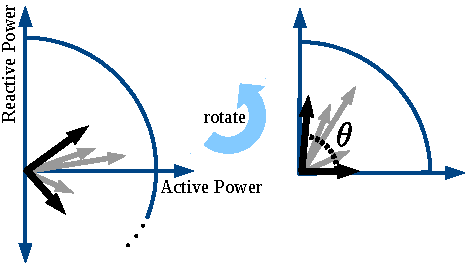
\includegraphics[scale=.8]{fig/rotate.pdf}
	\end{center} \vspace{-5pt}
\caption{Each vector represents a power demand $S_k$. The figure shows that the demands are rotated by the same angle. $\theta$ is the maximum angle between any pair of demands. }
	\label{fig:rotate}
\end{figure} 



Without loss of generality, this paper assumes that one of the demands, say $S_1$ is aligned along the positive real axis, and define a class of sub-problems, by restricting the maximum phase angle $\theta$ (i.e., the argument) that any other demand makes with $S_1$ (see Fig.~\ref{fig:rotate} for an illustration). Note that that in practice $\theta \le \frac{\pi}{2}$, because there are regulations that require electric equipment to conform with a certain maximum power factor (e.g., $\frac{P_k}{|S_k|}\ge 0.8$ \cite{NEC}). For the clarity of presentation, this paper assumes that $P_k \ge 0$ and $Q_k \ge 0$.


\begin{figure}[!htb]
	%\includegraphics[scale=0.3, trim = 0 0 0 0]{fig/normunif.png}
	\centering \vspace{-5pt}
	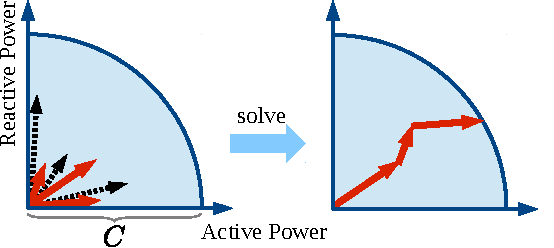
\includegraphics[scale=.7]{fig/fig-sol-horizontal.pdf} \vspace{-5pt}
\caption{The red vectors (thick arrows) represent a feasible solution to {\sc maxPA} such that the total magnitude of the red demands lies within the radius $C$.} \vspace{-5pt}
	\label{fig:problem}
 \end{figure}
 
%\begin{figure}[!ht]
%        \hspace{-10pt}      
%        \begin{subfigure}[h]{0.32\textwidth}\hspace{-10pt}
%                %\includegraphics[scale=0.3, trim = 0 0 0 0]{fig/normunif.png}
%                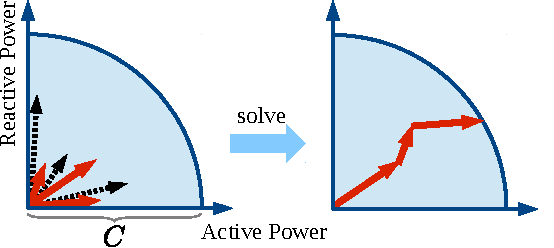
\includegraphics[scale=.7]{fig/fig-sol-horizontal.pdf}
%\caption{The left figure shows a set of all power demands $\{S_k(t)\}$. The red vectors (thick arrows) represent a feasible solution to {\sc maxPA} such that the total magnitude of the red demands remain within radius $C$ as shown in the right figure.}
%              	\label{fig:problem}
%        \end{subfigure}%
%        ~ %add desired spacing between images, e. g. ~, \quad, \qquad etc.
%          %(or a blank line to force the subfigure onto a new line)
%        \begin{subfigure}[h]{0.2\textwidth}
%              %  \includegraphics[scale=0.3, trim = 0 0 0 0]{fig/normnorm.png}
%              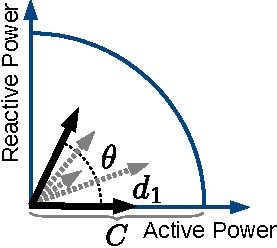
\includegraphics[scale=.7]{fig/fig-angle.pdf}
%\caption{The figure shows demands when all are rotated. The angle  $\theta$ is the maximum  between any pair of demands.\\ }
%	\label{fig:rotate}
%        \end{subfigure}
%\caption{Pictorial representations of {\sc maxPA}.}
%\end{figure}


An allocation $(x_k)_{k \in {\cal N}}$ can be equivalently represented by the set of satisfied customers $X \triangleq \{k\in {\cal N}\mid  x_k=1\}$. For a subset $X \subseteq {\cal N}$, denote $u(X) \triangleq \sum_{k\in X}u_k$.

%In particular, {\em polynomial-time approximation scheme} (PTAS) is an approximation algorithm with $1-\epsilon$ guarantee for any $\epsilon>0$.  The running time of a PTAS is polynomial in the input size for every fixed $\epsilon$, but the exponent of the polynomial might depend on $1/\epsilon$.  One way of addressing this is to define the {\em efficient polynomial-time approximation scheme} (EPTAS), whose running time is the multiplication of a function in $1/\epsilon$ and a polynomial in the input size independent of $\epsilon$. 
%An even stronger notion is a {\em fully polynomial-time approximation scheme} (FPTAS), which requires the running time to be polynomial in both input size and $1/\epsilon$. 








